\section{Computational Complexity}
Determining the complexity of a problem means giving bounds on the complexity of any possible algorithm for solving a problem.
We will focus on decision problems which is a class of problems for which the goal is to say, given an instance of the problem, if it has an answer or not. Other classes of problems that we will not explore are: Functional problems and optimization problems.\\
\begin{description}
    \item[Decision Problems] : 
    \item[Functional Problems] : 
    \item[Optimization Problems] :
\end{description}
Having a fast (polynomial) solution for an optimization problems implies that i have a fast one also for the Functional version and the decision version of the problem. The same goes inversely with the decision being hard, complex (non polynomial).\\
\subsubsection{Computation Model - Turing Machines}
The model of computation we are going to use to talk about computational complexity are Turing Machines which we are going to define here for ease of use.\\
\begin{definition}[Turing Machine]
    A Turing Machine is a quadruple $M= (K, \Sigma, \delta, s)$. Here K is a finite set of states; $s \in K$ is the initial state. $\Sigma$ is a finite set of symbols, we say $\Sigma$ is the alphabet of M. We assume that K and $\Sigma$ are disjoint sets. $\Sigma$ always contains the special symbols $\sqcup, \triangleright$: the blank and the first symbol o starting symbol. Finally $\delta$ is a transition function, which maps $K\times \Sigma$ to $(K \cup {h,"yes","no"})\times \Sigma \times {\leftarrow, \rightarrow,-- }$. We assume that h (the halting state), "yes" (the acceptin state), "no" (the rejecting state) and the cursor directions $\leftarrow, \rightarrow, --$, for "stay" are not in $K \cup \Sigma$. The function $\delta$ is the "program" of the machine. It specifies, for each combination of current state $q\in K$ and current symbol $\sigma \in \Sigma$, a triple $\delta(q,\sigma) = (p,\rho,D)$
\end{definition}
\begin{definition}[Configuration of a Turing Machine]
    We can define the operation of a Turing machine formally using the notion of a configuration. Intuitively, a configuration contains a complete description of the current state of the computation. Formally a configuration of M is a triple (q,u,w), where $ q \in K$ is a state, and $w,u$ are strings in $\Sigma^*$. $u$ is the string to the left of the cursor, including the symbol scanned by the cursor, and $u$ is the string to the right of the cursor, possibly empty. Finally q is the current state. 
\end{definition}

\subsubsection{Time Complexity}
This is a decision problem. There's a problem P, a class of models of computation M. The goal is to find in M the fastest machine m that solves P. By fastest we mean that executes least instructions. We need to fix a notion of dimension of the input which is usually done in the definition of the model of computation.\\
\begin{definition}[Time complexity for M TM, on input x]
    We say that M, Turing Machine, on input x has time complexity t if 
    \[ 
        (s,\triangleright, x) \underbrace{\longrightarrow}_{\text{t steps}} (H, w, u), \quad H\in {h,"yes","no"}
    \]
\end{definition}
\begin{definition}[Time complexity for M TM ]
    M has time complexity $f: \mathbb{N}\longrightarrow\mathbb{N}$ if:
    \[ 
        \forall x \in \Sigma^*\quad (s,\triangleright, x)\underbrace{\longrightarrow}_{\text{t steps}}(H,w,u) 
    \]
    with $t\leq f(|x|)$
    This definition is a worst case time complexity. 
\end{definition}
\subsubsection{URM}
We already know about turing machines but now we'll introduce Unlimited Registry Machines (URM):\\
Every URM has an infinite set of registers ($R_0, R_1, \ldots, R_n$), in any of these registers there can be an arbitrarily long natural number.
\begin{itemize}
    \item $S(i) \rightarrow R_i = R_i+1$.
    \item $Z(i) \rightarrow R_i = 0$.
    \item $T(i,j) \rightarrow R_j = R_i$.
    \item $J(i,j,k) \rightarrow if \;R_i = R_j$ jump to instruction k
\end{itemize}
Example, P:\\
Compute $x+1$. For the turing machine this means receiving the binary digits of $x$ and I want on output the result of $x+1$. The complexity is linear with the number of digits.\\
With the URM the complexity is 1, I just need $S(0)$. The problem is that we are hiding the size of the input so this model is not reasonable.\\
Let's make an addition to the URM model and add the instructions $P(i) \rightarrow R_i = R_i*R_i$ and we execute these instructions:
$T(0,1), J(1,2,6), P(0), S(2), J(3,3,2)$. The output goes: $x, x^2, x^4, x^8, \ldots x^{2^x}$ with complexity $\Theta(n)$. \\With a turing machine only writing the digits of the output requires at least $\Theta(2^xlog(x)) \leadsto \Omega(2^x) $.\\
\begin{definition}[Uniform complexity Cost]
    Each instruction of the models has complexity $\Theta(1)$. This is not reasonable when we are using models include operations that make the involved integers grow too fast. An example of this behaviour is the URM with the product operation.\\
\end{definition}
\begin{definition}[Logarithmic Complexity Cost]
    Each instruction of the models has complexity that depends on the number $k$ of digits it manipulates.\\
\end{definition}
It is clar that it's fundamental to analyze the complexity of all the instructions in your computational model. Let's do it for the URM model:
\begin{itemize}
    \item $S(i) \rightarrow R_i = R_i+1 \quad \Theta(log(R_i))$
    \item $Z(i) \rightarrow R_i = 0 \quad \Theta(1)$
    \item $T(i,j) \rightarrow R_j = R_i \quad \Theta(log(r_i))$
    \item $J(i,j,k) \rightarrow if \;R_i = R_j \text{ jump to instruction } k \quad \Theta(min(log(R_i), log(R_j)))$
    \item $P(i) \rightarrow R_i = R_i*R_i \Theta((log(R_i)^2))$
\end{itemize}
To decide when to use a Logarithmic criteria for computing the complexity cost I have to look for operations in the algorithm that in a polynomial number of steps makes the input grow exponentially, moreover these are used a number of times that depends on the size of the input.\\
If we now analyze the cost of the models with the Logarithmic complexity cost we get that the URM and the Turing machine are related.\\
\begin{thesis}[Computational Church Turing Thesis]
    All reasonable models of computation are polynomially related.
    \[ 
        M_1: \Theta(f(n)) \leadsto M_2: \Theta (p(f(n))), \quad p \; polynomial 
    \]
    In this case reasonable means that we have to use the logarithmic criteria.
\end{thesis}
We define as $ P = \{L | L \text{can be decided in polynomial time on a deterministic Turing Machine}\} $. P is invariant with respect to the model of compuation ( consequence of the extended Church tesis).
\subsubsection{Review of k-tape TM}
Later we'll now demonstrate that the loss in time complexity that we experience by moving from one reasonable model of computation to another is at most quadratic.\\
To show this result we reintroduce now some concepts about a k tape Turing Machine or k-TM. A configuration for a k-TM takes the following form
\[ 
    (q,w_1,u_1,w_2,u_2,\ldots,w_k,u_k),\quad w_i,u_i \in \Sigma^*
\]
Every $w_i$ is the string left of the cursor on k-th tape.\\ The initial configuration for a k-TM on input x is:
\[ 
     (s,\triangleright,x,\triangleright,\varepsilon,\triangleright,\varepsilon, \ldots,\triangleright,\varepsilon)
\]
A language $L\subseteq \Sigma^*$ is decided by a k-TM M if
\[ 
    \forall x \in \Sigma^* 
     \begin{cases}
        M(x) = "yes" & if \; x\in L \\
        M(x) = "no" & if \; x \notin L 
     \end{cases}
\]
A language $L\subseteq \Sigma^*$ is accepted by a k-TM M if
\[ 
    \forall x \in \Sigma^* 
     \begin{cases}
        M(x) = "yes" & if \; x\in L \\
        M(x)\uparrow & if \; x \notin L 
     \end{cases}
\]The difference is that a machine that accepts a language diverges if the input is not in the language. In fact, for a machine that does not terminate on input x we write$ M(x) \uparrow $ and we say it diverges while the notation for a terminating TM is $ M(x) \downarrow $.\\
The notion of computation: a computation step for a machine M is a binary relationship between two configuration: \[ 
    (q, u_{1},w_{1}, \ldots,u_{k},w_{k}) \longrightarrow (q^{'},u_{1}^{'},w_{1}^{'}, \ldots,u_{k}^{'},w_{k}^{'})
\]
(For reference Papadimitriu section 2.1)
%%%%%%%%%%%%%%%%%%%%%%%%%%%%%%%%%%%%%%%


\subsection{Time Complexity}
\begin{definition}[Time complexity]
    Given M a k-TM and x the input for M, we say that M on input x takes time $t$ if
    \[ 
        (s, \triangleright, x, \triangleright, \varepsilon, \ldots, \triangleright, \varepsilon) \longrightarrow ( H,\ldots) 
    \] 
    with $ H \in {yes, no, halt} $. We say that M operates in time at most $ f(n) $ if: \[ 
    \forall x with |x| = m \quad M on x takes time at most f(|x|) 
    \]. Here $( H,\ldots)$ is short for final configuration.
\end{definition}
\begin{definition}[Time complexity classes]
    Given a language $L \subseteq \Sigma^*$, L is decidable in $ TIME(f(n))$ if and only if  $\exists k-TM M$ that decides L and operates in time at most $f(n)$.
    \[ 
        TIME(f(n)) = \left\{ L \mid L\subseteq \Sigma^* \exists M k-TM\; s.t. \; \text{M decides L in time } f(n) \right\} 
    \]
    Example: L is the language of all strings that are palindromes. $ \Sigma = \{0,1\}\cup\{\sqcup, \triangleright\} $ we get $ \Theta(n^2) $
\end{definition}
\subsubsection{Polynomial relationship between models of computation}
We can first start looking at this relationship by showing the time complexity for the problem of deciding the language of palindromes on a 1-TM and a k-TM. Here we summarize the program ideas:
\begin{description}
    \item[1-TM]: We suppose that the tape is originally $\triangleright, x_{1}, \ldots,x_{n}, \sqcup$. The machine starts reading the first character $x_1$, stores the information about the digit in its state, replaces $x_1$ with $\triangleright$ then moves right until it finds $\sqcup$. At this point it goes back one step and confronts the character from the state and the one under the cursror. If they match it goes back all the way to the new $\triangleright$ and starts over, otherwise it rejects.
    \item[k-TM]: Starting from the first character the machines reads the value and copies it on a different tape, all the way to $x_n$. After it copied all the input it moves back to the start on either of the tape and starts moving one cursor forward and one backwards meanwhile checking for matching character at every step.
\end{description}

\begin{theorem}[Theorem 2.1 Papadimitriu]:\\
Given M a k-TM that operates in time f(n), then there exists a 1-TM M' operates in time at most $ \Theta(f(n)^2) $ such that $\forall x \quad M(x) =M'(x)$. Fundamental hypothesis is that $f(n)\geq n$
\begin{proof}
    For the sake of brevity we'll only give the idea for the proof. Basically M' has to mimic the k tapes of M with it's only tape. To do that we specify an alphabet that is $\Sigma \cup \munderbar{\Sigma} \cup \left\{ \triangleright', \triangleleft \right\}$. We will use the underlined characters to store the information of where is the cursor on the k-th tape of the machine M and the special starting symbol will be use to delimit the start of every k-th string, meanwhile the $\triangleleft$ delimits the end of each k-th "tape".\\
    To perform any steps of M, M' will have to scan the entire tape once to store in its state the information about every symbol under the k-th cursor and once more to perform the necessary modifications, needing in total 4 traversals of the entire tape. Particular attention must be given to the case in which the k-th cursor is on the last symbol of its sub-tape and wants to move to the right. To allow for such a move we must shift the entire string starting by marking the tape end symbol with an underbar $\munderbar{\triangleleft}$, then going all the way to the end of the tape of M' and shifting every character one position. We can now move back to $\munderbar{\triangleleft}$, move it to the right as $\triangleleft$ and placing $\sqcup$ in its previous position.
\end{proof}
\end{theorem}

%
%Papadimitriu 2.8.4
%\[ 
%    \forall n \exists x s.t. K(x) \geq l(x)
%\]
%Exercie 2.8.5\\
%Show that the language of palindromes cannot be decided in $ \omega(n^2) $  less than %quadratic time over a 1-TM. (look for Luca trevisan article about it). The idea: you take n %= |x| and the string:
%\[ 
 %   x_{1}, \ldots,x_{n}\underbrace{00000}{0}x_{n}, \ldots,x_{1}
%\]

\begin{theorem}[Speed-up Theorem ]
    If $L \in TIME(f(n))$ , then \[ 
        \forall \epsilon > 0,\quad \exists L \in TIME(\epsilon \cdot f(n)+n+2) 
    \]
    The multiplicative constant in front of the higher degree term is dependant on the model of computation.
    \begin{proof}
        Idea: M' will have to process many digits in a signle "macro" step to reduce the mulitplicative constants.
        Hypothesis:\\
        $L \in TIME(f(n)) \rightarrow \exists M k-TM$ decides L in time $f(n)$
        Demonstration:\\
        \[ 
            \exists M'\; 2-TM\; \text{ decides L in time } f'(n)=\varepsilon \cdot f(n)+n+2, \quad \forall \varepsilon >0
        \]
        $M'$ has to simulate $m$ steps of $M$ with a constant number of steps (around 6 steps on $M'$ constitute a macro-step of $M'$) ($m$ will depend on $\varepsilon \leadsto \frac{7}{m})$.\\
        $M$ will make $f(n)$ steps to complete the computation while the steps of $M'$ will be $6 \cdot \frac{f(n)}{m}$\\
        $M$ in $m$ steps can at most read and change $m$ symbols on the tape. So if $M'$ prime has to fit into a single step the $m$ steps of the $M$ machine, its alphabet will have to be $\Sigma^m$.This means that we will encode $m$ symbols of the alphabet of M into a single symbol of the alphabet of M'\\
        Each slot of the tape of $M'$ contains an element of the alphabet $\Sigma^m$.\\
        A key point is to understande that $M$ with $m$ steps can at most change slots of its tape that were grouped into 2 different slots of the $M'$ machine.\\
        At the beginning of the computation $M'$ reads the input x and encodes it into tuples of $\Sigma^m$.
        In order to simulate the $m$ steps of $M$ the machine $M'$ reads the current tuple, the one on the left and the one on the right and it stores that information on the state. Then it changes at most 2 of the three tuples.\\The multiplicative constant 6 comes from the number of moves $M'$ has to make (these can be optimized):
        \begin{itemize}
            \item Read the information on the starting tuple and store it in the state and move to the left
            \item Read the information and store it in the state and move back to the starting tuple
            \item Move to the right tuple 
            \item Read the information and store it in the state, move back to the starting tuple
            \item Change the symbol on the tape and move to either the right or left tuple
            \item Change the symbol on the tape 
        \end{itemize}
        The $n$ additive term is because $M'$ has to read the string x of $M$ and encode it in blocks of $m$, and it has to read the start symbol and blank space of the tape of $M$ which are the 2 steps. Finally $M'$ has to move back to its starting position so there are an additional $\frac{n}{m}$ steps.\\
        $TIME(f(n))$ only makes sense with $f(n) \geq n$
    \end{proof}
\end{theorem}

\subsection{Space Complexity}
\begin{definition}[Space Complexity]
    Suppose that, for a k-string Turing Machine M and input x, computation of M
    \[ 
        (s,\triangleright, x, \ldots, \triangleright, \varepsilon) \overset{M^*}{\longrightarrow} (H, w_q, u_1, \ldots, w_k,u_k) 
    \] where $H \in \left\{ h, "yes", "no" \right\}$ is a halting state. Then the space required by M on input x is $\sum_{i=1}^{k}{\absolute{w_i}+\absolute{u_i}}$. If, however, M is a machine with input output (I/O TM), then the space required by M on input x is $\sum_{i=2}^{k-1}{\absolute{w_i}+\absolute{u_i}}$.\\
    Suppose now that $f$ is a function from $\mathbb{N}$ to $\mathbb{N}$. We say that Turing Machine M operates within space bound $f(n)$ if, for any input x, M requires at most $f(\absolute{x}) $.\\
    Finally, let L be a language. We say that L is in the space complexity class SPACE($f(n)$) if there is a Turing Machine with input output that decides L and operates within space bound $f(n)$. 
\end{definition}
I/O turing machines are linearly related to a generic k-string Turing Machines, so we'll use I/O machines to talk and determine space complexity and generic k-string Turing Machines for time complexity.
\begin{theorem}[Space Speed Up Theorem]
    $L \in SPACE(f(n)) : \forall \varepsilon >0 \; L \in SPACE(\varepsilon\cdot f(n) +2)$
\end{theorem}


\subsection*{RAM computational model}
A Random Access Machine, or RAM, is a computing device which, like the Turing Machine, consists of a program acting on a data structure. A RAM's data structure is an array of registers, each capable of containing an arbitrarily large integer, possibly negative. These registers are divided into working registers named $r_i$ and input registers $i_j$.\\
Formally a RAM program $P=(\pi_{1}, \ldots,\pi_{n})$ is a finite sequence of instructions, where each instruction $\pi_i$ is one of the following.
\begin{description}
    \item[READ J]: $r_0 = i_j$
    \item[READ $\uparrow$j] = $r_0 = i_{r_j}$
    \item[STORE J] = $r_j = r_0$
    \item[STORE $\uparrow$ j]  $r_{r_j}=r_0$
    \item[LOAD J] $r_0 = r_j$
    \item[LOAD $\uparrow$ j] $r_0 = r_{r_j} $
    \item[LOAD =j] $r_0 = j$
    \item[ADD] $r_0 = r_0+r_j$
    \item[ADD $\uparrow$ j] $r_0 = r_0+r_{r_j}$
    \item[ADD =j]    $r_0 = r_0+j$
    \item[SUB] $r_0 = r_0-r_j$
    \item[SUB $\uparrow$ j] $r_0 = r_0-r_{r_j}$
    \item[SUB =j]    $r_0 = r_0-j$
    \item[HALF] $r_0 = \left\lfloor \frac{r_0}{2} \right\rfloor$
    \item[JUMP j] $k = j$, (k is the program counter) 
    \item[JPOS j] if $r_0>0 $then $k = j$
    \item[JNEG j] if $r_0<0$ then $k = j$
    \item[JZERO j] if $r_0=0$ then $k = j$
    \item[HALT] $k=0$
\end{description}
%%%%%%%%%%%%%%%%%%%%%%%%%%%%%%%%%%%%%%%%%%%%%%%%%%%%%%%%
%Operational semantics: the meaning of a program is a graph with a starting configuration and a relationship between a different configuration.\\
%denotational semantics: you map the program to the function computed by P, static verification tecniques, abstract interpretation. Optional study reference Robin Milner Calculus of communication systems\\
%%%%%%%%%%%%%%%%%%%%%%%%%%%%%%%%%%%%%%%%
\begin{definition}[RAM configuration]
    A configuration of a RAM is a pair
    \[ 
        C=(k,R) 
    \]
    where k is the program counter and tells the instruction to be executed and R is the set of working and index regsiters with their content
    \[ 
        R = \left\{ (r_{j1}, j_{j}), \ldots,(r_{jk}, j_{k}) \right\} 
    \]
\end{definition}
\begin{definition}[Computation step]
    Let us fix a RAM program P and input $I = (i_{1}, \ldots,i_{n})$. Suppose that $C=(k,R)$ and $C'=(k', R')$ are configurations. We say that $(k,R)$ yields in one step $(k',R')$ , written $(k, R) \overset{P,I}{\longrightarrow} ( k', R')$, if the following holds: $k'$ is the new value of $k$ after the execution of $\pi_k$ the k-th instruction of P. R', on the other hand, is the same as R with the difference that registers involved in the $\pi_k$ instruction have to altered accordingly.\\
    For instance the program P is $P=(\pi_{1}, \ldots,\pi_{n})$ and the instruction $\pi_k = ADD j$ and $R={(r_{j1}, j_{1}), \ldots,(r_{jh }, j_{h}}$ from the configuration \[ 
    (k, R) \overset{P,I}{\longrightarrow} ( k+1,(R\setminus\{(r_0,r_0)\}\cup \{(r_0, r_0+r_j)\}) )
\]
\end{definition}
This completes the definition of the relation $\overset{P,I}{\longrightarrow}$. We can now define $\overset{P,I^k}{\longrightarrow}$ (yields in k steps) and $\overset{P,I^+}{\longrightarrow}$ (yields).
\begin{definition}[Function computed by RAM]
    Let P be a RAM program, let D be a set of finite sequences of integers, and let $\phi$ be a function from D to the integers. We say that P computes $\phi$ if, and for any $I \in D, (1,\emptyset) \overset{P,I^*}{\longrightarrow} (0,R)$, where $(0, \phi(I)) \in R$
\end{definition}

The RAM program P on input I takes time $t$ if $(1, \emptyset) \overset{P,I^t}{\longrightarrow} (0,R)$. We then say that
P operates in time $f(n)$ if $\forall I: l(I) = n $, P on I takes time $f(n)$ where $l(I) = \sum_{j=1}^{h}{l(i_j)}$ where $l(i_j)$ is the length of the binary representation of that integer $i_j$.
\subsubsection{Simulation of a Turing Machine with RAM}
Since the RAM only operates on integer we have to encode the alphabet of the TM into integers.
\[ 
    D_{\Sigma}= \{(i_i,\ldots, i_n,0) | n\geq 0 \forall 1\leq j\leq n \quad 1 \leq i_j\leq l,  \} 
\]
M decides $L \subseteq \Sigma^*$, while a RAM P simulates the Turing machine M (that decides L) if P computes the function  \[ 
    \phi_L : D_{\Sigma} \longrightarrow \mathbb{N}
\]where \[ 
    \phi_L : (i_{1}, \ldots,i_{n}, 0) = \begin{cases}
        0 & \sigma_{1}, \ldots,\sigma_{n} \notin L\\
        1 & \sigma_{1}, \ldots,\sigma_{n} \in L  
    \end{cases} 
\]
\begin{theorem}
    If $L \in TIME(f(n))$ there esists a program P that computes $\phi_L$ and P operates in O(f(n))
    \begin{proof}
        $M = (\Sigma, K, \delta, s)$ Turing machine needs to be simulated by a RAM program P. A generic intermediate step of the computation will present the following configuration:
        \begin{itemize}
            \item Register R0 will be used for the computation.
            \item Register R1 stores the name of the register containing the symbol that is read by the Turing machine at each step.
            \item Register R3 and following will store each one character contained on the tape of the Turing Machine.
        \end{itemize}
        At the beginning of the computation the RAM will have all registers empty and the input string on its input registers. Then it starts a loop copying the input numbers starting from register R3. The loop goes on if it reads from memory something different from 0. Finally it writes the number 3 in the R1 register to signal that the corresponding register is the one under the cursor.\\The program P will have a set of instruction to simulate every possible state $q \in K$. Each of these set is then divided into $k = \absolute{\Sigma}$ subsequences, each for every possible symbol. Suppose our generic step starts at instruction number $N_{q,\rho_j}$ and our generic step is $\delta(q,\rho_j) = (p,\rho_l,D)$\\
        \begin{enumerate}
            \item[$N_{q,\rho_j}$] LOAD $\uparrow 1$ \quad (fetch the symbol scanned by the cursor)
            \item[$N_{q,\rho_j+1}$] SUB = $\rho_j$ \quad (subtract j, the number of the symbol tested)
            \item[$N_{q,\rho_j+2}$] JZERO $N_{q,\rho_j+4}$ \quad (if the simbol is $\rho_j$ we have work to do)
            \item[$N_{q,\rho_j+3}$] JUMP $N_{q,\rho_{j+1}}$ \quad (otherwise, try next symbol)
            \item[$N_{q,\rho_j+4}$] LOAD = $\rho_l$ \quad ($\rho_l$ is the symbol written)
            \item[$N_{q,\rho_j+5}$] STORE $\uparrow 1$ \quad (write $\rho_l$)
            \item[$N_{q,\rho_j+6}$] LOAD 1 \quad (the position of the cursor)
            \item[$N_{q,\rho_j+7}$] ADD = d \quad (d is 1 if $D=\rightarrow$, -1 if $D=\leftarrow$, 0 if $D=-$)
            \item[$N_{q,\rho_j+8}$] STORE 1
            \item[$N_{q,\rho_j+9}$] JUMP $N_{p,\rho_1}$ \quad (start simulation of state p)
        \end{enumerate}
        One instruction of M is simulated on P with at most $9 \times \absolute{\Sigma} $instructions which is $O(f(n)) + O(n)$, the additional linear term is to set up the machine. As always we need to add the hypothesis $f(n) \geq n$.
    \end{proof}
\end{theorem}
\subsubsection{Simulating a RAM with a Turing machine}
\begin{theorem}
    If we have a RAM program P that computes a function $\phi$ in time f(n), then there exists a 7-tape Turing Machine with I/O M that computes the same function in time $O((f(n))^3)$
    \begin{proof}
        First tape is for input and last tape for output of course. The second tape is used to store the content of the registers R, it constists of a sequence of strings of the form $b(i):b(r_i)$ separated by ';' and possibly sequences of blanks.Each time the value of Register $i$ is updated, the previous $b(i):b(r_i)$ pair is erased (we overwrite them with $\sqcup$) and a new pair is attached at the end of the tap, shifting the end symbol $\triangleleft$ accordingly.The third tape stores the program counter k of P while the other three tapes are used for the arithmetic operations.\\\\
        How many instructions of M do I need to simulate one instruction of P?\\
        How long is the content of the tapes of M during the simulation?\newline
        Let's focus on the instruction $ADD \uparrow j: \quad r_0 = r_0+r_{r_j}$. We start scanning the 2nd tape and copy the content of $r_0$ on the 4th tape. A second scan is needed to find the content of the register $r_j$ and copy the content on the 6th tape.\\
        Then I scan the second tape again to find the register whose name is written on the 6th tape, I copy its content on the 5th tape.\\ I compute the sum operation between the content of the 4th and 5th tape and write them on the 6th tape.\\
        After this i must go on the 2nd tape, find the register $r_0$, substitute it and its content with blanks, move all the way to the end of the tape and add the new pair $r_0$ with its updated content.\\
        For every instruction we use a constant number of scans of the 2nd tape. To estimate the number of instruction of M needed to simulate P we then must find out how long at most the 2nd tape is during the computation.\\ To answer this question we must understand how long a single pair $(i,r_i)$ of P can be after t steps? Let's denote as B the biggest constant (number used for immediate operations), and its length $l(B)$
        \begin{lemma}
            After t steps of P $i$ and $r_i$ can have length at most 
            \[ 
                l(I)+l(B)+t 
            \]Summing two numbers we can at most produce a new number that has 1 more bit
        \end{lemma}
        Each of the pairs on the 2nd tape is long at most $2*(\underset{n}{l(I)}+\underset{const.}{l(B)}+f(n))$. Keeping in mind the assumption $f(n)\geq n$ each of the pair is $O(f(n))$. After f(n) steps we can at most have f(n) of these pairs. Putting together these two observation we can say that the content of the 2nd tape during the computation is long at most $O(f(n)^2)$.\\ One instruction of P requires $O(f(n)^2)$ steps to be simulated by M. So if M needs to simulate f(n) instructions of P the total is $O(f(n)^3)$ instructions of M.
    \end{proof}
\end{theorem}

\subsection{Non-deterministic Turing Machine}
\begin{definition}[Nondeterministic Turing Machine]
    A Nondeterministic Turing Machine is a quadruple $N = (K,\Sigma, \Delta,s)$.\\Contrarily to its deterministic counterpart $\Delta$ is no longer a function from $K\times \Sigma$ to $(K\cup\left\{ h,"yes","no" \right\})\times \Sigma \times \left\{ \leftarrow,\rightarrow,- \right\}$ but instead a relation $\Delta \subset (K\times \Sigma)\times \left[ (K\cup\left\{ h,"yes","no" \right\})\times \Sigma \times \left\{ \leftarrow,\rightarrow,- \right\} \right]$. That is, for each state-symbol combination there may be more than one appropriate next steps, or none at all. 
\end{definition}
We define N.D. T.M configurations just as we did for their deterministic counterpart with the exception that "yields" is no longer a function and is instead a relation and a computation step is a subset of the cartesian product of the configurations. We define as degree of nondeterminism of a configuration the number of valid configurations that are obtained with a single computation step.\\The computation of N over input x can be expressed as tree (more formally a DAG) and we say that N accepts x if and only if at least one of its computation sequences terminates with "yes". Inversely we say that N rejects x if and only if all computation sequences terminate with "no".
\begin{figure}[htbp]
    \centering
    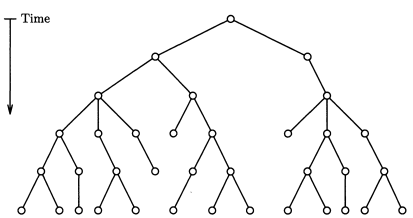
\includegraphics[width=10cm]{Complexity/ndtm-computation-tree.png}
\end{figure}\\
We define $f(n)$ as the function that produces as output the height of the computation tree of N over input x. We say that N operates on input x in time $f(n)$. 
\begin{definition}[Time complexity of N.D. T.M]
    A N.D. T.M is said to work in time $f(n)$ if it has time complexity over the input x $\forall x \in \Sigma^*$ at most $f(n)$ such that $\absolute{x}=n$.
\end{definition}
\begin{definition}[Decidability of a language over N.D. T.M.]
    A N.D. T.M. N decides a language L if $\forall x \in \Sigma^*$
    \[ 
        \begin{cases}
            \text{if } x\in L \text{ then there exists a computation of N over x that terminates with yes} \\
            \text{if } x\notin L \text{ then all the computations of N over x terminate with no} 
        \end{cases}
    \]
\end{definition}

\subsubsection{Complexity classes}
We define the time complexity class P of the languages that can be decided in polynomial time over a deterministic Turing Machine as follows:
\[ 
    P = \bigcup_{k\in \mathbb{N}}{TIME(n^k)}
\]We remember that a language belongs to this class regardless of the model of computation used, as long as it was reasonable, this is a consequence of the Extended Church-Turing thesis. Then we continue defining the time complexity class NP of the languages that can be decided in polynomial time over a nondeterministic Turing Machine:
\[ 
    NP = \bigcup_{k\in \mathbb{N}}{NTIME(n^k)}
\]The relationship between these two classes has been in discussion for decades and is still uncertain. Something we can say for sure is that $P \subseteq NP$ as we can always think of a deterministic TM as a nondeterministic TM which always has degree of nondeterminism equal to 1.
\begin{theorem}
    Suppose that language L is decided by a nondeterministic TM N in time $f(n)$. Then it is decided by a 3-tape deterministic Turing Machine M in time $\mathcal{O}(c^{f(n)})$, where $c> 1$ is some constant depending on N. Using complexity class notation we can restate this result in the shorter form:
    \[ 
        NTIME(f(n)) \subseteq \bigcup_{c>1}{TIME(c^{f(n)})} 
    \]
    \begin{proof}
        We can think of the exaustion of all possible computation step sequences as a series of choices leading to a final state. Any of this series is a sequence of integers in the range [0,d-1], (d-1 being the height of the computation tree). The simulating machine M has to visit in post-order the computation tree of N. This tree has at most $d^{f(n)}$ nodes where d is the highest degreee of nondeterminism of any of the configurations. This means that a "fast" deterministic model, like a program in C, will visit the tree in linear time with respect to its size $d^{f(n)}$. A deterministic TM will take at most $(d^{f(n)})^b$ where b is the highest degree of the polynomial relationship between our "fast" model and a standard deterministic machine. 
    \end{proof}
\end{theorem}
\begin{definition}[Space complexity of a N.D. T.M.]
    Given a k-tape nondeterministic Turing machine with input and output $N=(K, \Sigma, \Delta, s)$ we say that N decides language L within space $f(n)$ if N decides L and, for any $x\in (\Sigma-{\sqcup})^*$, if $(s,\triangleright,x,\ldots,\triangleright,\varepsilon) \overset{N^*}{\longrightarrow}(q,w_1,u_1,\ldots,w_s,u_s)$ then $\sum_{j=2}^{s-1}{\absolute{w_iu_i}}\leq f(\absolute{x})$. That means that we require that N, under no cirumstances, uses space in its "scratch" strings greater than function $f$ in the input length. 
\end{definition}
We can then define the space complexity class $NSPACE(f(n))$ as the set of all languages that can be decided by a N.D. T.M. using space $f(n)$.

\section{Undecidability of Halting Problem}
Proof based on the existence of Universal Turing machines, trhough enumeration of TM done by diagonalization. (Look at Quantum Computing since Dam) Read chap 3 of Papadimitriu

\section{Relationships between complexity classes}
Complexity classes are defined by fixing the following:
\begin{itemize}
    \item A model of computation (TM)
    \item A mode of computation (deterministic or non-deterministic)
    \item A resource to measure (time, space ecc...)
    \item A function used as a bound
\end{itemize}
Regarding the last point: the function f(n) used must at least be computable but we'll see that this is not enough. We'll se that $ \exists f computable \quad TIME(f(n)) = TIME(2^{f(n)}) $ when we cover the GAP theorem. We'll also see the Hierarchy Theorem that in short says: \\
If f is proper, then $TIME(f(n)) \subsetneq TIME(f(n)^3)$
\begin{definition}[Proper complexity function]
    Idea: not only f needs to be computable, but to compute f(n) must be computable with not more than f(n) time and space.\\
    Formally, a function $ f: \mathbb{N}\longrightarrow \mathbb{N} $ is proper if: \begin{itemize}
        \item f is non-decreasing
        \item $ \exists M_f k-TM$ with I/O such that $ \forall x with \absolute{x}= n $
        \[ 
            (s,\triangleright, x ,\triangleright, \varepsilon, \ldots, \triangleright, \varepsilon) \overset{M_f,t}{\longrightarrow}(halt, \underset{\triangleright \times \sqcup}{x_1, x_2}, \triangleright, \sqcup^{j_2}, \ldots,  \underset{f(x) \text{ in unary}}{\triangleright \sqcap^{f(\absolute{x})}}, \sqcup) 
        \]
        and $ t = O(n+f(n))$, $j_i = O(f(n)) \forall i= 2, \ldots,k-1$ and $t, j_i$ do not depend on x. 
    \end{itemize}
    The additional n term in the time complexity is because we are defining a set of functions that are bound for both TIME and SPACE complexity definition. In the case of TIME it is only reasonable to look for function that are at least linear, but with space we can also have less than that. If f and g are proper, also $f+g$, $f\times g$, $f^g$, $f(g(n))$ are all also proper
\end{definition}
\begin{definition}
    A TM M is precise if $\exists f,g \mid \forall n\geq 0 \forall x | \absolute{x} = n $ M(x) terminates after f(n) steps using space g(n). 
\end{definition}
\begin{property}
    If $L \in TIME(f(n))$ and f is proper then there exists M precise that decides L in time $\mathbf{O(f(n))}$ ( So not exactly f(n), but precisely $O(f(n))$).
    \begin{proof}
        $L \in TIME(f(n)) \leadsto M'$ decides L in f(n) but M' is maybe not precise. So we build a new machine that works as follows:\\
        We take all the necessary inputs for $M_f$ the machine that computes f because it is proper and each time M' makes a step it deletes one of the 1's produced in output (in unary) from $M_f$ after having computed f(n). This way if i realize that for that specific input x the machine terminates early i know how many steps to waste doing nothing so that it ends after exactly f(n) steps. ( Read proof in the book and find the mistake)
    \end{proof}
\end{property}
\subsection{Complements of Non-deterministic classes}
If C is a complexity class (either det. or nondet., space or time), we define:
\[ 
    co-C = \left\{ \bar{L} \mid L \in C \right\} 
\]Pay attention that $co-C \neq \bar{C}$\\\\
$P = U_{k\in\mathbb{N}}TIME(n^k)$, and we have a language $L \in P$ it means that $\exists M det. TM$ that decides L, we can easily get $\bar{L}$ by inverting accepting and rejecting states of M to get $\bar{M}$ that decides $\bar{L}$ and $\bar{L} \in P$
\begin{itemize}
    \item co-P = P
    \item TIME(f(n)) = co-TIME(f(n))
    \item SPACE(f(n)) = co-SPACE(f(n))
\end{itemize}
\subsection{Hierarchy between complexity classes}
Taking $L \in NP$ and $x \in L$, it means that in its computation tree over x there exists a leave terminating with yes. It necessarily means that $x\notin \bar{L}$. We cannot simply invert the final states to get a nondet. TM that decides $\bar{L}$, we get a TM, it works in f(n) but it doesn't decide the complement. For this reason we cannot classify the relationship between NP and co-NP.
\begin{theorem}[Hierarchy Theorem]
    Halting problem: $H = \left\{ M;x \mid M(x) \downarrow \right\}$.\\ Two main results: the halting problem is recursively enumerable, H is not recursive (theorems from chapter 3). \\
    $H_f = \left\{ M,x \mid \text{M accepts x in at most } f(\absolute{x}) steps \right\}$ if f is proper $H_f \in TIME(f(n)^3)$ and $H_f\notin TIME(f(n))$
\end{theorem}
The Hierarchy theorem really proves that the class P is a union of languages that belong to different polynomial time classes and there isn't a highest degree polynomial into which I can embed all other problems.
\begin{lemma}
    $H_f \in TIME(f(n)^3)$ if $f$ is proper.
    \begin{proof}
        $U_f$ takes in input the encoding of machine M and the encoding of x in binary and we call this length n. On a second tape we copy x in $O(f(n))$. By definition of proper function there exists $M_f'$ that computes $f'$ since $f'$ is proper. This machine will compute in binary $f'(f(x))$ in unary in a different tape. It will do it in $O(f(n))$ steps. On a different tape, the machine $ U_f $ will need to store the configuration of M and to perform the simulation of one step $U_f$ will need a constant number of scans of the first tape and the configuration tape. The machine $U_f$ has to simulate $O(f(n))$ steps of M. Then to measure the steps required for each simulated step we need to find the length of the configuration tape as the input is of length n by definition. Each of the strings in the configuration tape has length $f(n)$ because M can at most write that many symbols in the same amount of steps for each tape. If we say that $k_m$ is the constant representing the number of tapes of M. At any step of the simulation, the configuration tape is long $O(k_m\cdot f(n))$ which is certainly $O(f(n)^2)$ ( we are even exagerating, just to be safe). Putting all together we have that $U_f$ decides $H_f$ in $O(f(n)^3)$ steps which means $H_f \in TIME(f(n)^3)$
    \end{proof}
\end{lemma}
\begin{lemma}
    $H_f \notin TIME(f(\lfloor \frac{n}{2}\rfloor))$
    \begin{proof}
        By contraddiction:
        \[ 
            \exists M_{H_f} \text{ decides } H_f \text{ in at most } f(\lfloor \frac{n}{2}\rfloor) \text{steps}
        \]
        Consider D, $D(M) = yes$ if and only if $M_{H_f}(M;M) = no$\\
        $D(M) = $yes iff $M(M) = no$ or $M(M)\uparrow$ or $M(M)=yes$ after more than $f(\absolute{x})+5\absolute{x}+4$ steps.\\\\ How much time is required by D? It receives M as input and wants to exploit the powerful machine $M_{H_f}$ so it needs to produce on the second tape the correct input (M,M), after having that D behaves exactly like $M_{H_f}$ and complements the result. $M_{H_f}$ will terminate in $f(\lfloor\frac{2n+1}{2}\rfloor) = f(n)+5n+4$ (ATTENTION THAT THE BOOK DOESN'T ADD THIS SUPPLEMENTARY TERMS REQUIRED TO COPY THE INPUT ON THE SECOND TAPE TWICE)\\\\
        Which is the result of $D(D)$?\\
        If we assume D(D)= no then $M_{H_f}(D;D) = $yes, but this means that $D;D \in H_f$ which would require that D(D)= yes. This is a contraddiction. To prove the contraddiction we also need the other case: D(D) = yes then $M_{H_f}(D;D) =$no, this means that $D;D \notin H_f$ and that happens either because $D(D)\uparrow$ or because $D(D) = $ yes in more than $f(\absolute{D})+5\absolute{D}+4 $ steps. This shows contraddiction in every case giving us our proof.
    \end{proof}
\end{lemma}
\begin{theorem}[Hierarchy]
    If $f(n)\geq n$ is proper then $TIME(f(n)) \subsetneq TIME(f(2n+1)^3)$. The inclusion is trivial while we have proof that it is not equal because the halting language over $m = 2n+1$ is included on the right and not the left. 
\end{theorem}
Remember $P = \bigcup_{k\in \mathbb{N}}{TIME(n^k)}$ we define $ExP = \bigcup_{k\in \mathbb{N}}{TIME(2^{n^k})}$. As a corollary we have that \[ 
    P \subsetneq ExP 
\]
\begin{proof}
    $P\subseteq TIME(2^n) \overset{Hierarchy}{\subsetneq} TIME((2^{2n+1})^3) \subseteq TIME(2^{n^2}) \subseteq ExP$
\end{proof}
\begin{theorem}[Gap Theorem]
    $\exists f$ recursive such that 
    \[ 
        TIME(f(n)) = TIME(2^{f(n)}) 
    \]Observation: f is not proper. It proves that non proper function exists.\\
    \begin{proof}
        We consider an enumeration of the Turing machines $M_{0},M_{1}, \ldots,M_{n},\ldots$.\\
        $P(i,k)$ iff $\forall M_h with h\leq i \forall x with \absolute{x}=i$, $M_h(x)$ terminates in at most k steps, or $M_h(x)$ terminates in more than $2^k$ steps, or $M_h(x) \uparrow$. $P(i,k)$ is decidable.\\
        Consider (we want to define f(i)) the interval $k_1 = 2i, k_2 = 2^{k_1}, \ldots k_j = 2^{k_{j-1}}+1$
        N(i) number of possible input s of length i for the machines $M_0, M_1, \ldots, M_i$ and it's $\Sigma_{h=0}^{i}{\absolute{\Sigma_h}^i}$\\
        For a given input x of length i the machine $M_h$ either does not terminate or it terminates in $s_{xh}$ steps. If we consider N(i) +1 intervals there is at least one in which we do not have any of the number $s_{xh}$'s. We take that interval, suppose it starts at $k_l$ and we define $f(i)=k_l$ and f is computable. $P(i,f(i))= P(i,k_l)$ and f(i) has been defined so that $P(i,k_l)$ is true.\\
        We then need to prove that $L \in TIME(2^{f(n)}) \Rightarrow L \in TIME(f(n))$.\\\\
        Since $L\in TIME(2^{f(n)})$ it means that L is decidable and there is a machine $M_j$ that decides L in at most $2^{f(n)}$ steps. $\forall x with \absolute{x}= i \quad i\geq j$ our machine $M_j$ is among the first $M_i$: $M_0, M_1, \ldots, M_j, \ldots, M_i$. $M_j$ since is terminating in at most $2^{f(i)}$ it has to terminate in at most $f(i)$. We get that $M_j$ decides L in $TIME(f(n))$
    \end{proof}
\end{theorem}
\begin{theorem}
    If $f$ is proper then:
    \begin{align*}
        PSPACE(f(n)) &\subseteq NSPACE(f(n)) \\
        TIME(f(n)) &\subseteq NTIME(f(n)) \\
        TIME(f(n)) & \subseteq PSPACE(f(n)) \\
        PSPACE(f(n)) &\subseteq TIME(c^{f(n)+\log{n}})\\
        NTIME(f(n)) & \subseteq PSPACE(f(n)) \\
        NSPACE(f(n)) &\subseteq TIME(c^{f(n)+\log{n}})
    \end{align*}
    \begin{proof}
        \[ 
             L \in NTIME(f(n)) \Longrightarrow L\in PSPACE(f(n))
        \]
        If $L \in NTIME(f(n)), \exists N$ non-deterministic TM that decides L in time $f(n)$. This means that there exists M deterministic TM that decides $L$ in time $O(c^{f(n)})$. Let's recall that N uses at most $f(n)$ space because it's working in $f(n)$ space. The tape used by M to store the nondeterministic choices to simulate N requires at most $f(n)$ characters, each $1 \leq c_i \leq d$ and requiring $\log{d}$ (constant) space. So M is working in space $O(f(n))$ because with respect to N it is only adding $\log{d}\cdot f(n)$ space.
    \end{proof}
    \begin{proof}
        \[ 
            L \in NSPACE(f(n)) \Longrightarrow L \in TIME(c^{f(n)+\log{n}})
        \]
        Since $ L \in NSPACE(f(n)), \exists N$ nondeterministic I/O TM that decied L in space $f(n)$. We have to look at the work performed by N as a set of configurations:
        \begin{align*}
            &\qquad\tikznode{1}{$(q_1, w_{1}^1,u_{1}^1, \ldots,u_{k}^1,w_{k}^1)$}\\
            &\qquad\tikznode{2}{$(q_2, w_{1}^2,u_{1}^2, \ldots,u_{k}^2,w_{k}^2)$}\\
            \tikznode{0}{$(q,w_1,u_1,\ldots,w_k, u_k)$}&\qquad \vdots \; d\\
            &\qquad\tikznode{d}{$(q_n, w_{1}^d,u_{1}^d, \ldots,u_{k}^d,w_{k}^d)$}\\
        \end{align*}
        \begin{tikzpicture}[remember picture,overlay,rounded corners,>=stealth,shorten > =1pt,shorten <=1pt,thick]
            \draw[->] (0.east) |- (1.west);
            \draw[->] (0.east) |- (2.west);
            \draw[->] (0.east) |- (d.west);
        \end{tikzpicture}We can fix input the input x and $\absolute{x} = n$. We can modify how we write the configurations and we can substitute $w_1^i, u_1^i$ since the input tape is fixed and we only need the integer $j$ of the position of the cursor on the input tape. We further modify the configuration removing $w_k^i,u_k^i$ because given that the machine is I/O we cannot go back and read/modify the content. Now we calculate how many possible configurations of the form $(q,j,w_2^i,u_2^i,\ldots,w_{k-1}^i,u_{k-1}^i)$ of N on input x are possible:
        \begin{align*}
            &\underset{states}{(\absolute{K}+2)} * \underset{\text{cursor positions}}{n+2} * \prod_{i=2}^{k-1}{\underset{\text{contents of tape } i}{\left( \absolute{\Sigma}^{f(n)} \times \absolute{\Sigma}^{f(n)} \right)}}=\\
            &=(\absolute{K}+2) * {n+2} * \absolute{\Sigma}^{2f(n)\cdot(k-2)}
        \end{align*}
        I now construct a deterministic machine M that will create the computation graph of N and then M has to decide whether the starting configuration is able to reach a node whose state is "yes".\\
        M produces the graph $G_N(x)$ in linear time with respect to $\absolute{G_N(x)}$. M solves a reachability problem over $G_N(x)$ in polynomial time w.r.t. $\absolute{G_N(x)}$, being generous let's say $\absolute{G_N(x)}^{10}$. We know that from our previous computation that $\absolute{G_N(x)} = (\absolute{K}+2) * {n+2} * \absolute{\Sigma}^{2f(n)\cdot(k-2)} = (\absolute{K}+2) * O(b^{f(n)+\log{n}})$. Then the reachability problem becomes $O(c^{f(n)+\log{n}})$ and c depends on N.
    \end{proof}
\end{theorem}
The problem with the last proof is that c depends on N so it changes depending on the language and of course the machine. For this reason the complexity relation is only partially correct because it isn't the same c for every language.
\begin{corollary}
    \[ 
        \tikznode{L}{L} \subseteq NL \subseteq \tikznode{P}{P} \subseteq  NP \subseteq \tikznode{PSPACE}{PSPACE} \subseteq \tikznode{NSPACE}{NSPACE} \subseteq ExP \subseteq NExP \subseteq \ldots
    \]
\end{corollary}
\begin{corollary}
    \[ 
        NSPACE(f(n)) \subseteq SPACE(c^{f(n) +\log{n}})
    \]
\end{corollary}
\begin{theorem}[Savitch Theorem]
    The problem \textsc{Reachability}$\in SPACE((\log{n})^2)$.
    \begin{proof}
        We define a predicate $Path(x,y,i)$ true when x reaches y in at most $2^i$ steps. For this we define a base case $Path(x,y,1)\; iff \; x =y \vee x \rightarrow y$
        \[ 
            Path(x,y,i+1) \Longleftrightarrow \exists z: Path(x,z,i) \wedge Path(z,y,i) 
        \]
        The machine receives in input the encoding of the graph, x and y. x reaches y if and only if $Path(x,y, \absolute{V})$. On the working tape we write down recursive calls and they accumulate like the stack of a recursive program. At most $\log{\absolute{V}}$ calls will accumulate and each of them is long at most $\log{\absolute{V}}$. This means that we can solve \textsc{Reachability} in $PSPACE((\log{n})^2)$
    \end{proof}
\end{theorem}
\begin{corollary}[Savitch Corollary]
    \[ 
        NSPACE(f(n)) \subseteq SPACE(f(n)^2),\quad f(n) \geq n
    \]
    \begin{proof}
        We have a computational graph $G_N(x)$ of size $b^{f(n)+\log{n}}$, using Savitch theorem we get
        \[ 
            SPACE((\log{b^{f(n)+\log{n}}})^2) = SPACE((f(n)+\log{n})^2)
        \]
    \end{proof}
    This proof is cheating a little because it doesn't account for the space required to create and compute the graph.
\end{corollary}

Another corollary to Savitch theorem
\begin{corollary}
    \[ 
        NSPACE = PSPACE 
    \]
    The classes are close enough that the speed up theorem allows us that they are the same
\end{corollary}

\subsubsection*{Relation between complement classes}
We want to explore the question:
\[ 
    CO-NSPACE(f(n)) ? NSPACE(f(n)) 
\]
To answer this we will use another result.\\
Problem:\\
Given $ G=(V,E) $ and $u \in V$ we want to compute the number of nodes reachable from u
\[ 
    \absolute{Reach_G(u)} 
\]
Recall the meaning of complement: $\bar{L} \in co-l, x \in \bar{L} iff x\notin L iff N(x)$ always terminates with no ( N non-det for L)
\begin{theorem}[Immerman - Szelepscényi]
    The problem of computing the number of nodes reachable from x in G can be solves in non-deterministic space $O(\log{n})$. ( We don't say this is in NL because this is not a decision problem, but a functional one). In the computational graph all the nodes terminating the computation correctly will output a number and that is the same and also the correct one. All other computation branches will terminate with "no" ( just a convention, we don't want a number)
    \begin{proof}
        S(i) is the set of nodes reachable from x in at most i steps.\\
       $ S(0) = \{x\}, \quad \absolute{S(0)}=1$. At each step we store $\absolute{S(k-1)}$ and use it to compute $\absolute{S(k)}$ for $k = 1,2,\ldots, \absolute{V}-1$\\
       Inside the loop for k we have another loop always startin with $l:=0$ for $u = 1,2, \ldots, \absolute{V}$:
       \begin{itemize}
        \item if $\underset{how?}{u \in S(k)} l=l+1$
        \item m:=0, reply:= false (if u in S(k) becomes true)
        \item for (v = 1,2,..., |V|) \begin{itemize}
            \item if(v in S(k-1))
            \item   m= m+1
            \item   if((v,u) in E)
            \item       reply:= true
        \end{itemize}
       \end{itemize}
       at the end if m < |S(k-1)| return "no", else return reply. During the computation we only store k, l, u, m, v, reply, |S(k-1)|, p and $w_p$. They all range between 1 and |V| so they all require logarithmic space so the whole problem is O(log\{n\})
    \end{proof}
\end{theorem}
\begin{corollary}
    If f is proper $f(n) \geq \log{n}$ 
    \[ 
        Co-NSPACE(f(n)) = NSPACE(f(n)) 
    \]
    \begin{proof}
        $\bar{L} \in Co-NSPACE(f(n))$ we want to prove $\bar{L} \in NSPACE(f(n))$
        If $L \in NSPACE(f(n))$ it means that there is N that decides L. $x \in \bar{L}$, i generate the graph $G_N(x)$ and check that "yes" is not reachable, count all the reachable nodes with Immerman-Szelepscényi. Terminate with "yes" iff during IS the node (yes) of the graph $G_N(x)$ is never reached and IS has terminated with a number
    \end{proof}
\end{corollary}
Exercises
7.4.5 NP closed under $\cup$ and intersection\\
7.4.6 $L^* = \left\{ w_{1}, \ldots,w_{n} | k\geq 0 , w_i \in L \right\}$. Prove that both P and NP are closed for the operator kleenstar:
\[ 
    L \in P \Rightarrow L^* \in P 
\]
7.4.7 $NP \neq SPACE(n)$ (use some closure under some operations to prove)\\

\subsection{Reductions}
Given two languages L1 and L2, suppose we have a fast (polynomial) algorithm for deciding L2. A reduction is a clever way to modify, adapt the algorithm for L2 in order to decide L1. We say that
\[ 
    L1 \preceq L2 
\]
L1 is reducible to L2 if I have a function $R:(\Sigma_1)^* \longrightarrow (\Sigma_2)^*$ such that $x \in L_1$ if and only if $R(x) \in L2$ and R is computable in logarithmic space.\\
If we have three languagnes $ L1 \preceq L2 \preceq L3 $ it is also true that $L1 \preceq$
\begin{proof}
    \[ 
        L1 \preceq L2 \Rightarrow R_1: (\Sigma_1)^*\longrightarrow(\Sigma_2)^* 
    \]
    \[ 
        L2 \preceq L3 \Rightarrow R_2: (\Sigma_2)^*\longrightarrow(\Sigma_3)^* 
    \]
    Consider $R1 \circ R2 : (\Sigma_1)^* \longrightarrow (\Sigma_3)^*$
    \[ 
        R_1 \circ R_2 (x) \in L_3 iff x \in L_1 
    \] We only need to prove that $R1 \circ R2$ is computable in logarithmic time. The first application of $R_1$ is fine and is $O(log(n))$. The second function takes input of lenght m (the length of the output of $R_1$). The size m is polynomial with respect to n so $O(log(m)) = O(k\cdot log(n))$. This is not enough. When the machine M2 requires $y_j$ the machine M1 produces $y_{1}, \ldots,y_{j}$ reusing the same cell.
\end{proof}
\begin{definition}[Closure by reduction]
    A class C is closed by reduction if $L \in C$ and $L' \preceq L$, then $L' \in C$. 
\end{definition}
\begin{definition}[Problem completeness]
    L is complete for C if
    \[ 
        L \in C and \forall L' \in C \quad L'\preceq L 
    \]We say that L is C-complete.\\
    One question we might ask ourselves: Is there a problem that is complete for P? NP?
\end{definition}
\begin{property}
    If C and C' are closed for reduction, L is C-complete and C'-complete then $C = C'$
\end{property}
\begin{property}
    If C and C' are such that $C \subseteq C'$ and are closed for reduction and L' is C'-complete and $L' \in C$ then $C = C'$
\end{property}
\textbf{Example:}
3-coloring, we have an undirected graph $G=(V,E)$ undirected. Each node has to be a color between White, Red or Green. If $\left\{ u,v \right\} \in E$ then $color(u) \neq color(v)$\\\\
SAT, Decide whether a boolean formula is satisfiable\\\\
$3-col \preceq SAT$: I consider 3 boolean variable for each node $u \in V$: $W_u, R_u, G_u$ and at least one of them must be true
\[ 
    \wedge_{u \in V}{W_u \vee R_u \vee G_u} \wedge 
\]but also that at most one of them must be true
\begin{align*}
    \wedge_{u \in V}&(W_u \rightarrow (\neg R_u \wedge \neg G_u)) \wedge \\ 
    & (R_u \rightarrow (\neg W_u \wedge \neg G_u)) \wedge \\ 
    & (G_u \rightarrow (\neg R_u \wedge \neg W_u))
\end{align*}
We need to ensure that each edge has nodes with different colors
\[ 
    \wedge_{u \in V}{(W_u \rightarrow \neg W_v) \wedge(R_u \rightarrow \neg R_v) \wedge(G_u \rightarrow \neg G_v)}
\]
G is 3-col if and only if R(G) is SAT, and this is computable in
\begin{lemma}
    $L \in C-complete$ if and only if $\bar{L} \in coC-complete$
    \begin{proof}
        Hp: $L \in C-complete$ Th:$\bar{L} \in coC-complete$\\
        $ L \in C \Rightarrow \bar{L} \in coC $. Let $L' \in co-C$, then $\bar{L'} \in C$ which implies
        \[ 
            \bar{L'} \preceq L \Rightarrow R:(\Sigma')^* \rightarrow (\Sigma)^* 
        \]$x \in \bar{L'}$ if and only if $R(x) \in L$, this means that $x \in L'$ if and only if $R(x) \in \bar{L}$ which brings us to the final conclusion $L' \preceq \bar{L}$
    \end{proof}
\end{lemma}
\subsection*{Complete problems}
Recall that a P-complete language means that $L \in P$ and $\forall L' \in P \quad L' \preceq L$. Boolean circuits: a DAG 
\begin{itemize}
    \item each node is either 0, 1, a variable, not, or, and
    \item Nodes of the type 0,1,variable do not have incoming edges
    \item Nodes of type not have only 1 incoming edge
    \item Nodes of type or, and have 2 incoming edges
    \item There is 1 node without outgoing edges
\end{itemize}
Circuit value:\\
Given a circuit without variable nodes the problem is to decide whether the circuit has value 1\\
Circuit SAT: \\
Given a circuit decide whether there exists an assignement for the variables such that the circuit has value 1\\
We'll now see that the first one will be a P-complete problem and the second one a NP-complete problem. The result we will study is the Levi-Cook theorem.
\begin{theorem}[Circuit Value P-completeness]
    Circuit Value is P-complete
    \begin{proof}
        First step I need to prove that Circuit is in P.  We need to visit the DAG using topological sorting and this can be done in polynomial time.\\
        Secon step I need to know that given $L\in P$ it has to be possible to $L \preceq CircuitValue$. If $L \in P$ it has to be true that $\exists M$ that decides L in time at most $n^k-2$\\ I can define a table $T_M(x)[i,j] \in \Sigma \cup (\Sigma \times K)$. $T_M(x)[i,j]$ only depends on
        \begin{itemize}
            \item $T_M(x)[i-1,j-1]$ 
            \item $T_M(x)[i-11,j]$
            \item $T_M(x)[i-1,j+1]$
        \end{itemize}This dependance is on the value of the cells, not the position i,j, this means that the same three values somewhere else on the table produce the same cell result. This dependance can also be seen as a boolean function $F_M:\left( \left\{ 0,1 \right\}^l \right)^3 \longrightarrow \left\{ 0,1 \right\}^l$. I can then split this function in l parts, each computing the h-th bit of the output. All of these partial functions can be seen as boolean circuits, each producing one bit of the binary encoding of the output.
        $T_M(x)$ can be built using $O(n^k \times n^k)$ copies of $C_M$. $C_M(x) = 1 iff x\in L$. $C_M$ is computable in logarithmic space on a different I/O machine, at every moment the machine only needs to remember i and j to know which copy of $C_M$ i am producing in output. Each of the indexes i and j only require logarithmic space.
    \end{proof}
\end{theorem}

\begin{theorem}[Circuit SAT NP-completeness]
    Circuit SAT is NP-complete
    \begin{proof}
        Circuit SAT $\in$ NP. If $L \in NP$ there exists a non deterministic machine N. I use the same idea as the previous theorem but we need to define the table for the non-deterministic machine N. We need to add a number of boolean variable to each row for every non-deterministic choice that i can make for every row.
    \end{proof}
\end{theorem}

Alternative definition of NP: A relation $ R \subseteq \Sigma^* \times \Sigma^*$ that is polynomially decidable. We say that R is polynomially balanced if $\exists k \; \forall (x,y) \in R \quad \absolute{y} \leq \absolute{x}^k$

\begin{theorem}
    $L \subseteq \Sigma^* \quad L \in NP$ if and only if $\exists R$ polynomially decidable and polynomially balances such that
    \[ 
        L = \left\{ x \mid \exists y (x,y) \in R \right\} 
    \]
    The string y is called the certificate, it is one of the possible evaluation that makes the formula true.
    \begin{proof}[$\Rightarrow$]
        $ L \in NP \Rightarrow \exists N$ that decides L in polynomial time and N is non-deterministic. I consider the sequence R
        \[ 
            R = \left\{ (x,c_1, \ldots, c_m) \mid x \in L \quad N(x; c_1, \ldots, c_m) = yes \right\} 
        \]
        We can deterministically, in polynomial time, decide R by modifying N to take in input also the choices and N works by choosing every time the correct choices ($c_1, \ldots, c_m$)
    \end{proof}
    \begin{proof}[$\Leftarrow$]
        R is polynomially decidable and polynomially balanced, moreover $L = \left\{ x \mid \exists y (x,y) \in R \right\} $
        I need to construct a N non-det machine that decides L. On the first tape I non-deterministically generate the bits of the certificate y and then I behave like M checking if the pair x,y is in R
    \end{proof}
\end{theorem}

\begin{proposition}[3-SAT is NP-complete]
    3-SAT is the language of formulas with clauses involving at most 3 literals. A clause is a disgiunction of literals. A literal is either a boolean variable or its negation.\\\\
    Conjunctive Normal Form is a form for formulas that are as follows:
    \[ 
        C_1 \wedge C_2 \wedge \ldots \wedge C_k, \quad C_h \; clause 
    \]\\
    Disjunctive Normal Form:
    \[ 
        (C_1 \wedge \ldots \wedge C_m) \vee (\ldots \wedge \ldots) 
    \]
    It is easy (polynomial) to bring a formula to CNF but it's hard to decide its satifiability

    \begin{proof}
        $3-SAT \in NP$, this can be proven with certificate, I can present a formula Y that is in CNF and its evaluation $v:{p_{1}, \ldots,p_{m}} \longrightarrow{0,1}$\\
        $Circuit-SAT \preceq 3-SAT$
        \[ 
            C-circuit \mapsto Y_C \mapsto \bar{Y_C} \; \text{conjunction of clauses}
        \]
        $\bar{Y_C} = C_1 \wedge C_2 \wedge \ldots C_m$, each clause might have more than three literals. So if $C = (l_1 \vee l_2 \vee l_3 \vee l_4)$ I create a new variable $z = l_3 \vee l_4$ so C changes and now is $C = (l_1 \vee l_2 \vee z) \wedge ( \neg z \vee l_3 \vee l_4)$
    \end{proof}
\end{proposition}

\begin{proposition}[Independent Set is NP-complete]
    Given a graph G = (V,E), a set I of verteces is Independent if 
    $\forall u,v \in I \quad {u,v} \notin E$. Given a graph G, and $k \in \mathbb{N}$ decide if G has an Independent set such that $\absolute{I} = k$
    \begin{proof}
        Ind. Set $\in$ NP can be proven with a certificate (G,k; I). It can be checked, in polynomial time, that the certificate expressed as a possible set of nodes is indeed Independent and of size k. I now need to prove $3-SAT \preceq Ind.Set$. Given the 3-SAT formula $Y  = (C_1 \wedge \ldots \wedge C_h)$ and for example $C_j = (l_{1j} \vee l_{2j} \vee l_{3j})$\\
        Non ho capito una sega
    \end{proof}
\end{proposition}

\begin{proposition}[Clique is NP-complete]
    Given a graph G=(V,E), $C \subseteq V$ is a clique iff $\forall u,v \in V \quad \left\{ u,v \right\} \in E$. So given a graph G and integer k, the problem is to decide if there is a clique of size k
    \begin{proof}
        Clique is in NP and it can be proven with a certificate in the form of a set of nodes. We can prove, in polynomial time. The reduction comes immediately by taking the complement of E. The problem could now be seen as the one of finding a Independent set of size k. 
    \end{proof} 
\end{proposition}

\begin{proposition}[Sub-graph Isomorphism is NP-complete]
    Given two graphs $G_1, G_2$ check if there exists a subgraph of $G_2$ that is isomorphic to $G_1$.
    \begin{proof}
        We'll reduce to Clique 
    \end{proof}

\end{proposition}

\begin{proposition}[Integer Programming is NP-complete]
    Using 3-SAT
\end{proposition}
The non linear disequalities if with integer solutions are called the diophantine equations or 10th Hilbert problem and they are undecidable. While over the reals they are decidable.

\begin{proposition}[Knapsack is NP-complete 9.10]
    We are going to consider the decision version of this problem.
\end{proposition}
\begin{theorem}[9.4]
    Any instance of Knapsack can be solved in $O(n\cdot W)$. (the idea is that given an instance the amount of space required to express the instance is logarithmic with respect to the size of the instance). we can say that this problem is only polynomial with respect to a bound on the input. They are called pseudo-polynomial algorithms
\end{theorem}
Another category of problem is that of strongly NP-complete ones, they are NP-complete even with bounds on the involved integers

\subsection{L-complete problems - Chpt. 16}
Given two languages in $\mathbb{L}$, $L_1, L_2$ we can draw a reduction $L_1 \preceq L_2$.\
I take two strings, both within the alphabet $\Sigma_2^*$, one inside the language and one outside. The string $\alpha$ in $\Sigma_1^*$ is transformed as x (the string in L2) if $\alpha \in L_1$ otherwise as y if $\alpha \in L_2$
\begin{theorem}
    If $L \in \mathbb{L}$ with $L\neq \emptyset, L \neq \Sigma^*$ then L is $\mathbb{L}$-complete
\end{theorem}
\subsection{NL-complete problems - Chpt. 16}
We've seen that Reachability is in NL. We've also seen that co-NL = NL so Unreachability is in co-NL.
\begin{theorem}[Reachability is NL-complete]
    Reachability is NL-Complete
    \begin{proof}
        $L \in NL$ means that there is a machine N 
    \end{proof}
\end{theorem}
Corollary: if Reachability is in L, then L = NL

\begin{theorem}
    2-SAT is NL-complete
    \begin{proof}
        2-SAT in NL we demonstrate by adding a node for every literal in the clauses and its negation. I then create edges from the negation of one to the second one: if the clause is $p \vee q$ it can be seen as $\not p \rightarrow q$ identifying an edge on the graph. This creates a path of truth. If we have both a path from p to $\not p$ and one from $\not p$ to p, then the formula is not satisfiable. We get that 2-UnSAT is in NL which means that 2-SAT is NL.\\\\
        I then have to prove that 2-SAT is NL-complete
    \end{proof}
\end{theorem}




